
\section{Apparatus}
This experiment was carried out at the Idaho Accelerator Center (IAC), using their fast-pulsed linear accelerator, which is an L--band frequency (1300 MHz) electron linear accelerator.
It is capable of pulse widths ranging from 50 ps to 2 $\mu$s with a maximum energy of 44 MeV.
See section~\ref{beam} for the accelerator parameters used during the experiment.
Figure~\ref{fig:Facility} shows a top down diagram of the experimental arrangement.

\begin{figure}[h]
\centering
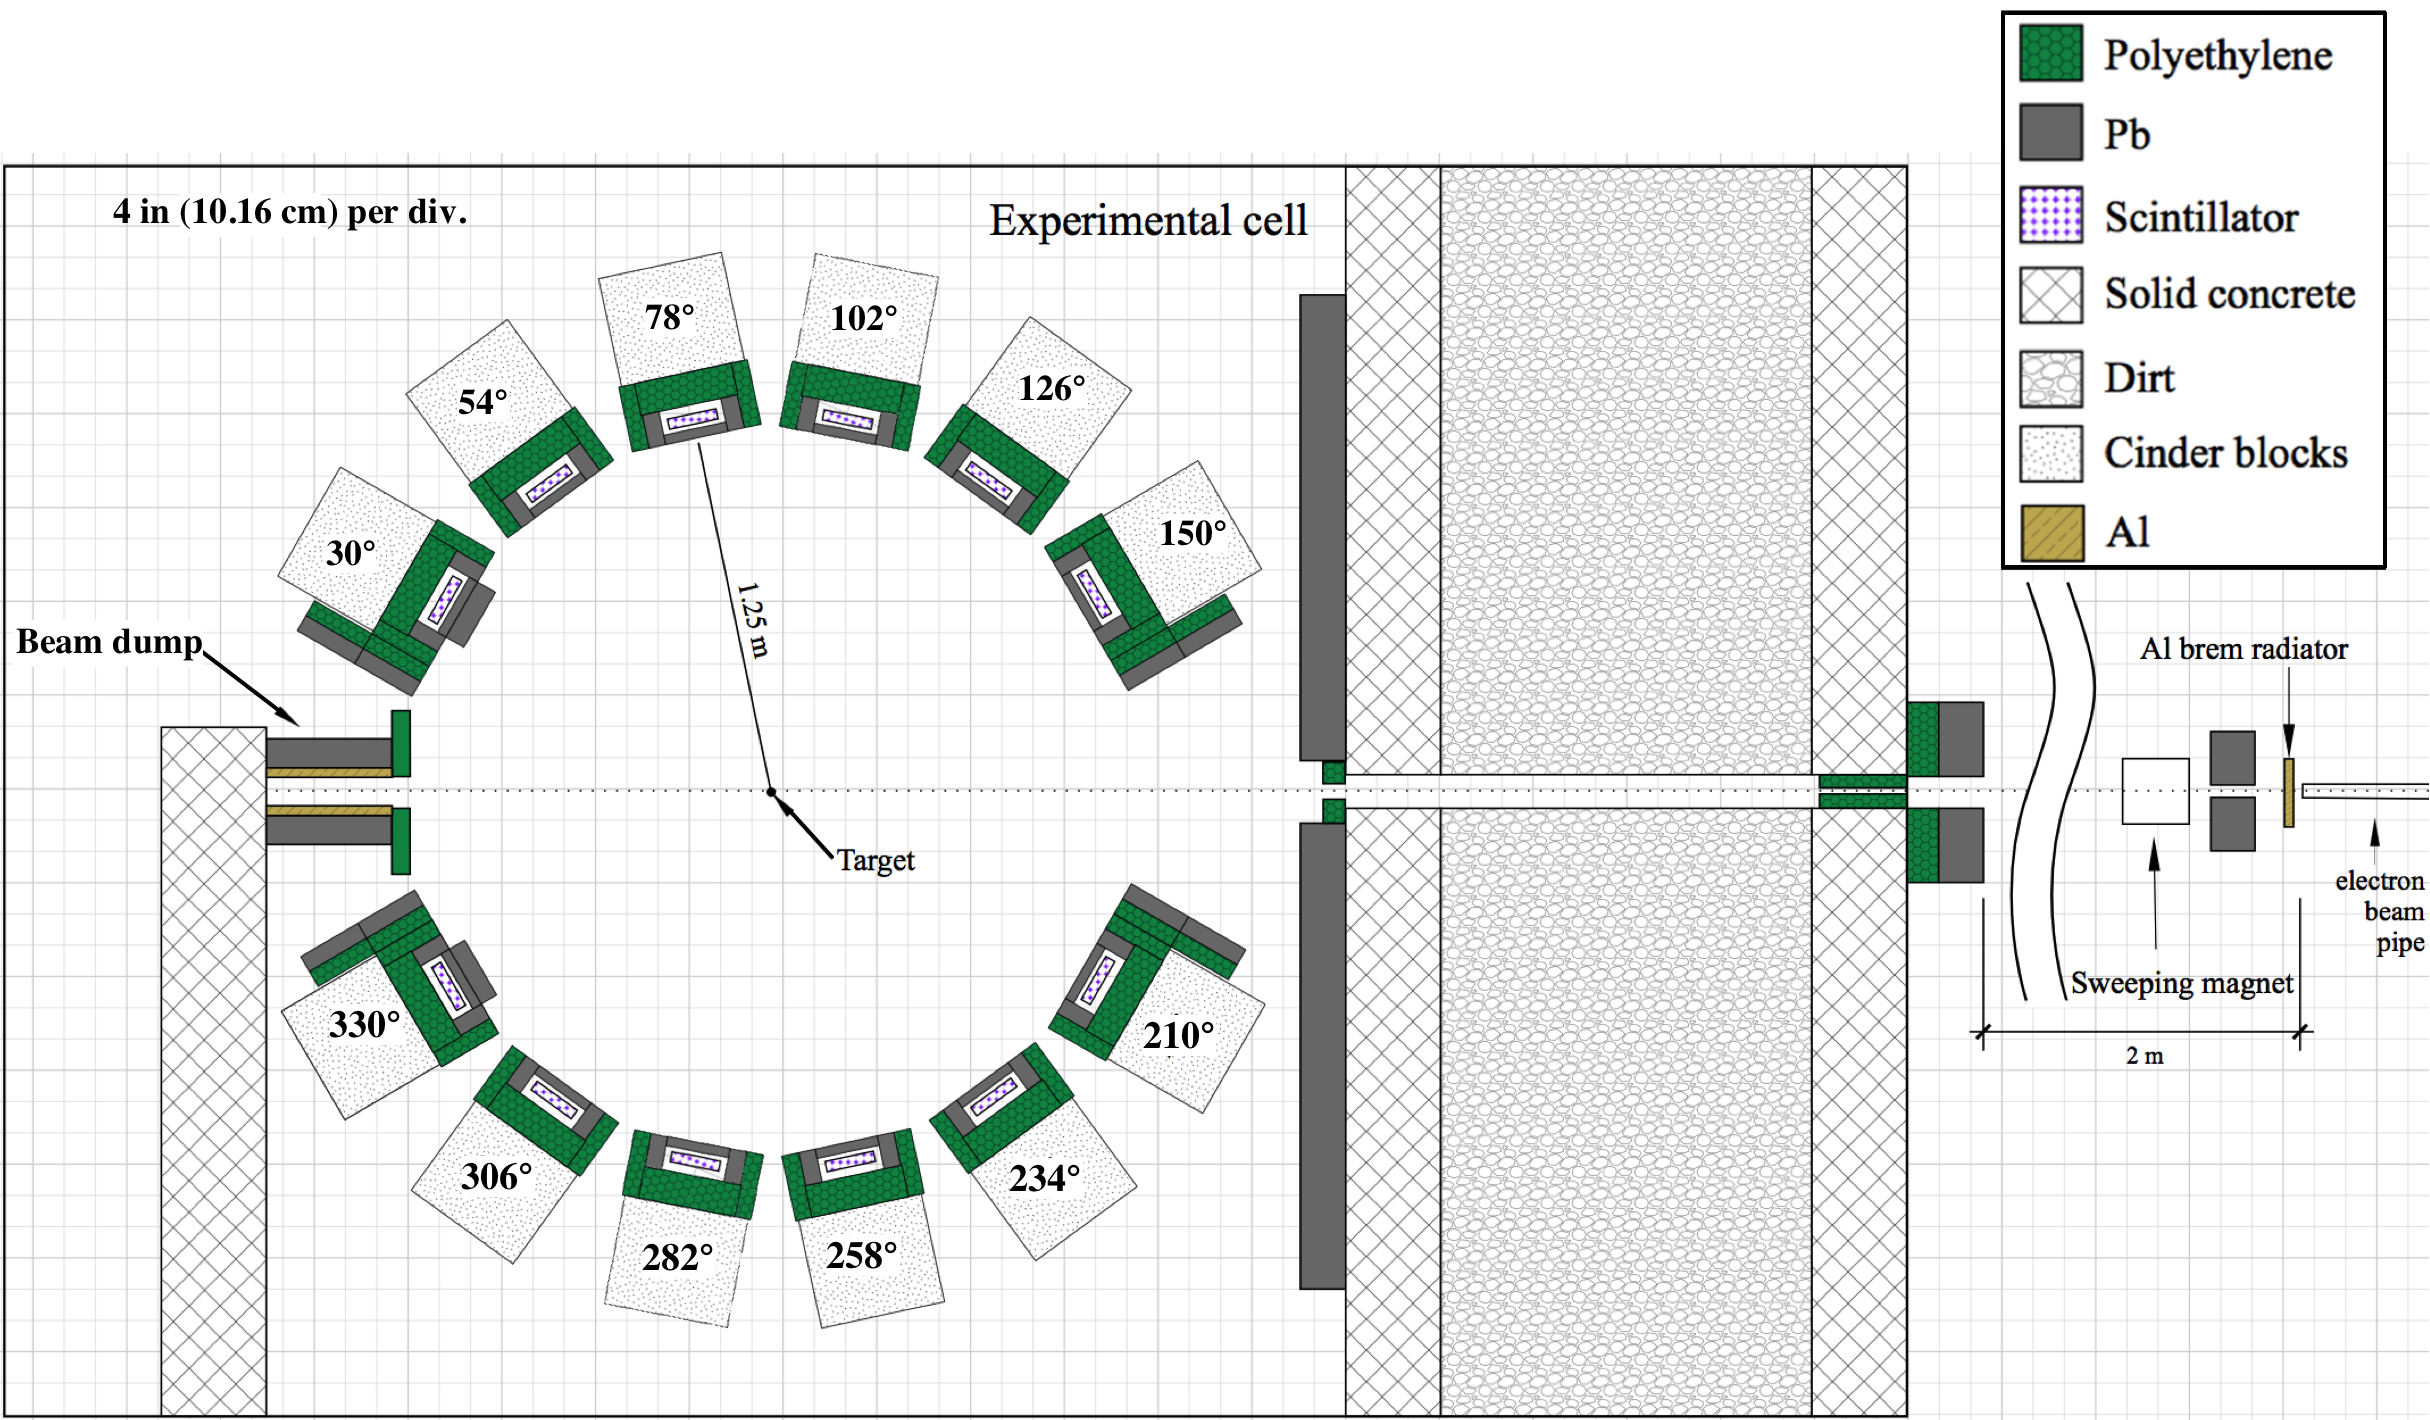
\includegraphics[width=0.95\textwidth]{Content/Methods/ExpArangment.jpg}
\caption{To-scale, top down diagram of the experimental setup.
An electron beam impinges upon a 3.8 cm thick Al radiator, and the resulting bremsstrahlung beam enters the experimental cell from the top.
The supporting structure for each detector has been labeled according to the angle, in degrees, between the center of each detector and direction of the incoming photon beam.
}
\label{fig:Facility}
\end{figure}
\subsection{Detectors}
\label{subsection:detectors}

The detection system measures neutron position and time of flight (ToF), which is defined as the time taken for a particle to travel from the target to a detector.
The purpose of the ToF measurement is to determine the kinetic energy of detected neutrons and to distinguish between photons and neutrons.
The detection system's positional precision is $\pm$9~cm, which gives an average angular precision of $\pm6^{\circ}$ in opening angle reconstruction.

The neutron detection system consists of fourteen shielded scintillators arranged in a ring around the target (see Fig.~\ref{fig:DetGeom}).
The scintillators were made from Polyvinyl Toluene (PVT), an organic plastic scintillator.
Attached to both ends of each scintillator are 10-cm long, non-scintillating, ultra-violet transmitting plastic light guides.
A Hamamatsu 580-17 photomultiplier (PMT) tube is fixed to each light guide using optical glue.
In order to increase the chance that scintillation light remains inside the scintillator, the scintillators were polished to remove micro-imperfections and were then wrapped in reflective aluminized mylar.

\begin{figure}[]
    \centering
    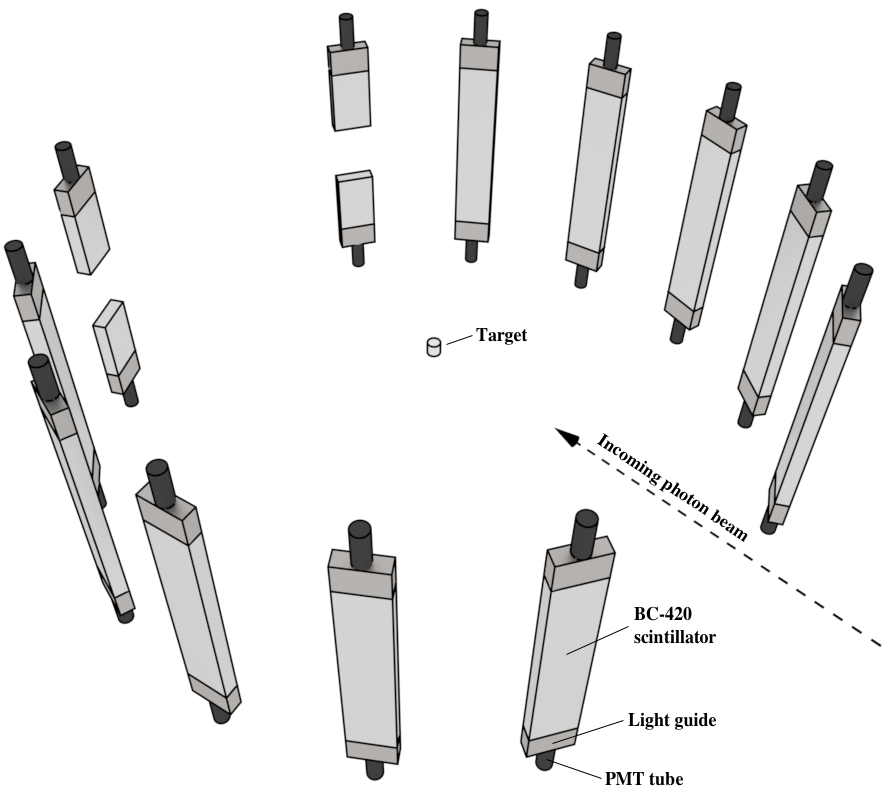
\includegraphics[width = 0.9\textwidth]{Content/Methods/Detectors.png}
    \caption{3-D render of the bare, unshielded scintillators, along with PMTs and light guides.}
    \label{fig:DetGeom}
\end{figure}

Ten out of the fourteen scintillators had dimensions of 76.2$\times$15.2$\times$3.8 cm$^3$.
The remaining four are the forward-most detectors, located at $\pm$ 30$^{\circ}$ with respect to the beam, and had dimensions of 25.4$\times$15.2$\times$3.8 cm$^3$.
These scintillators, 1/3 the size of the rest, are the result of the segmentation of two normally sized scintillators in order to address the high photon flux at these locations caused by the forward scattering of photons from the target.
Prior to segmentation, a photon was registered in the forward-most detectors at a rate of about 0.9 photons per pulse, and because the electronics were operated in single hit mode, this greatly reduced the effective neutron detection efficiency.
After segmentation, the photon detection rate was about 0.2 photons per pulse in each segmented detector.
The segmented detectors also differ from the rest in that they were instrumented with only a single PMT, and therefore provide a comparatively lower precision in energy and position measurements.
In order to test for systematic errors that may have resulted from the use of the segmented detectors, opening angle measurements were compared with and without their use, and the differences were well within experimental errors.

The relative efficiencies of the neutron detectors as a function of neutron energy were calculated by dividing measured and theoretical yields from the SF of $^{252}$Cf as according to MCNP.
The results are shown in Fig.~\ref{fig:RelErgEfficiency}, which uses the aggregate of events from all detectors, and in Fig.~\ref{fig:RelErgEfficiencyVariation}, which plots the result for each detector individually.
See section~\ref{Analysis} for a discussion of how the effects of detector efficiency are accounted for in this work.
\begin{figure}[]
    \centering
    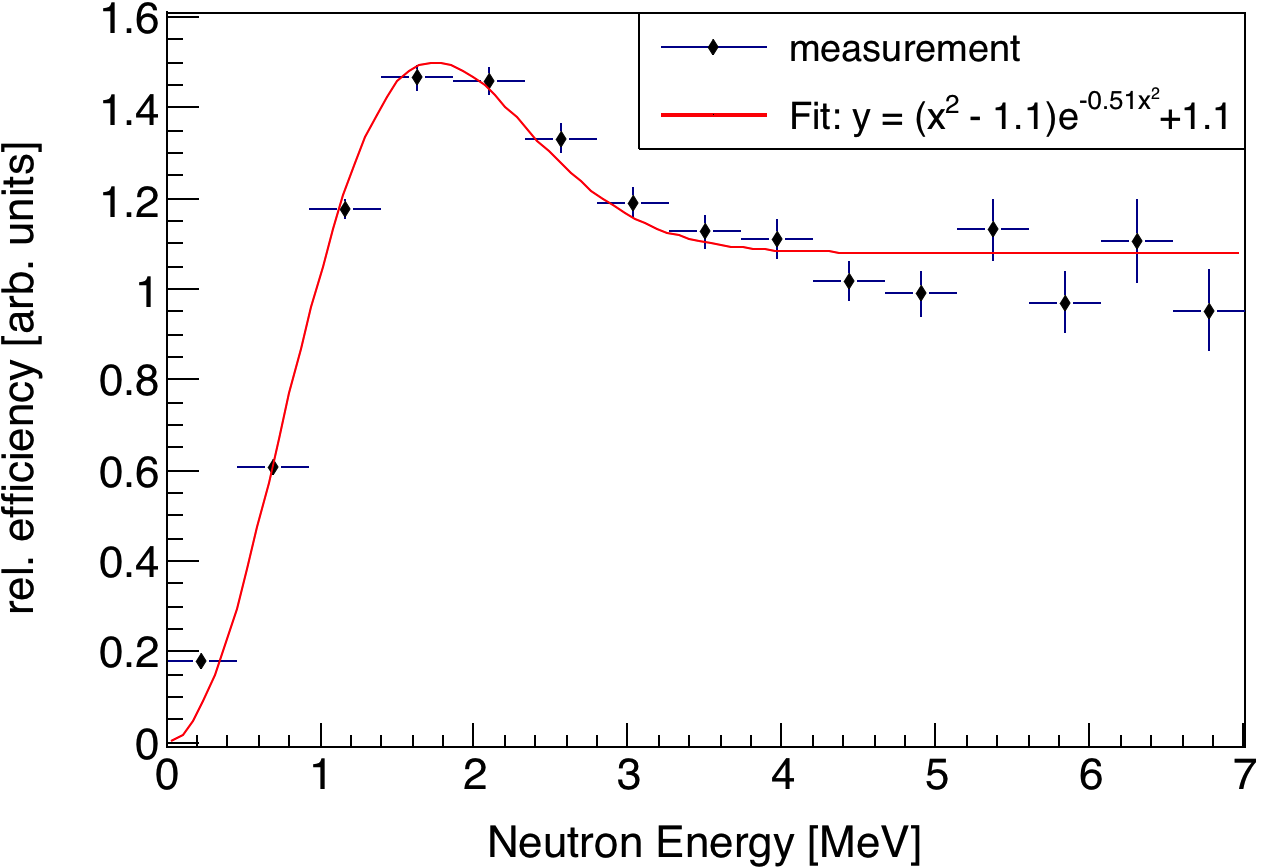
\includegraphics[width = 0.9\textwidth]{Content/Methods/RelErgEfficiency.png}
    \caption{The relative efficiency of the neutron detection system as a function of neutron energy is calculated by dividing the measured energy distribution by the theoretical energy distribution of neutrons from the SF of $^{252}$Cf.}
    \label{fig:RelErgEfficiency}
\end{figure}
\begin{figure}[]
    \centering
    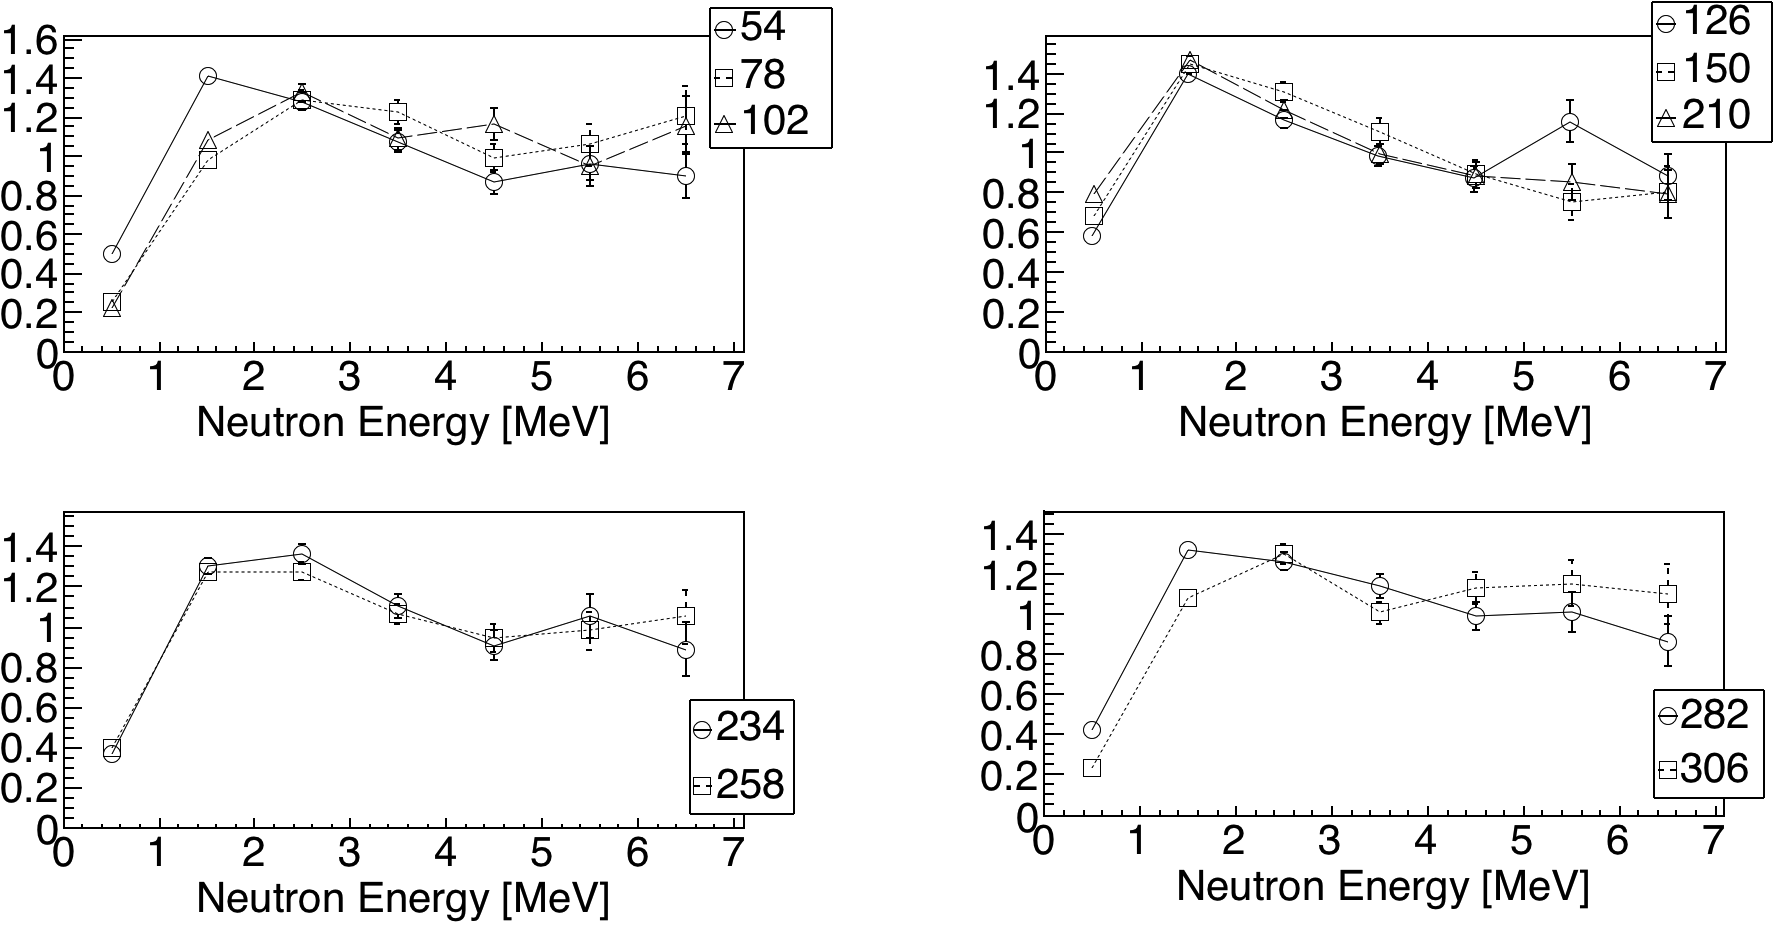
\includegraphics[width = 1\textwidth]{Content/Methods/RelErgEfficiencyVariation.png}
    \caption{
    The shape of the neutron detection efficiency curve varies among the detectors.
    The y-axis has arbitrary units and each curve is scaled to have the same integral.
    For the integrated neutron rates of each detector, see table~\ref{table:rates} in the appendix.
    Each detector is identified according to its angle relative to the photon beam, exactly as seen in Fig.~\ref{fig:Facility}.
    }
    \label{fig:RelErgEfficiencyVariation}
\end{figure}

\subsection{Detector Shielding}
\label{shielding}
The detector shielding, depicted in Fig.~\ref{fig:shielding}, was constructed using lead and polyethylene with the aim of reducing cross-talk, the detection of photons, and noise.
The sides of each scintillator were shielded with 5 cm of lead followed by 5 cm of polyethylene to reduce the chance of neutron cross-talk.
Lead was not placed behind the scintillators after an MCNP-POLIMI simulation indicated it would occur at significant rates otherwise.
Instead, 10~cm of polyethylene was placed behind the scintillators.
For a more detailed discussion about the issue of cross-talk, see section~\ref{crosstalk}.

The front face of each detector were subject to the highest photon flux due to the scatting of the Bremsstrahlung beam from the target.
The detection of a photon renders the given detector unable to detect any subsequent fission neutrons from the same pulse, due to the time needed for the detector to recover from the first event.
Lead mitigates this problem but has the side effect of scattering neutrons, and if a neutron scatters prior to being detected, the ToF measurement and position reconstruction will be incorrect.
The extent of measurement errors caused by this were quantified using an MCNP simulation, and accordingly, 2.5~cm of lead was placed along the front face of the detectors.
This diminished photon detection rates to reasonable levels (photon rates can be seen in table~\ref{table:rates}), and, according to the simulation, leads to a root-mean-square error in opening angle and ToF of 1$^{\circ}$ and 0.3~ns, respectively, due to neutron elastic scattering.

Because of the particularly high photon flux at the sides of all detectors located directly adjacent to the beam, an additional 2" of lead was placed along the sides of these detectors.
For the same reason, an additional 2" of lead was also placed and along the front faces of the detectors farthest downstream, located at $\pm30^{\circ}$ from the beam line.
The differences in shielding design among the detectors can be seen in Fig~\ref{fig:Facility}.
\begin{figure}
    \centering
    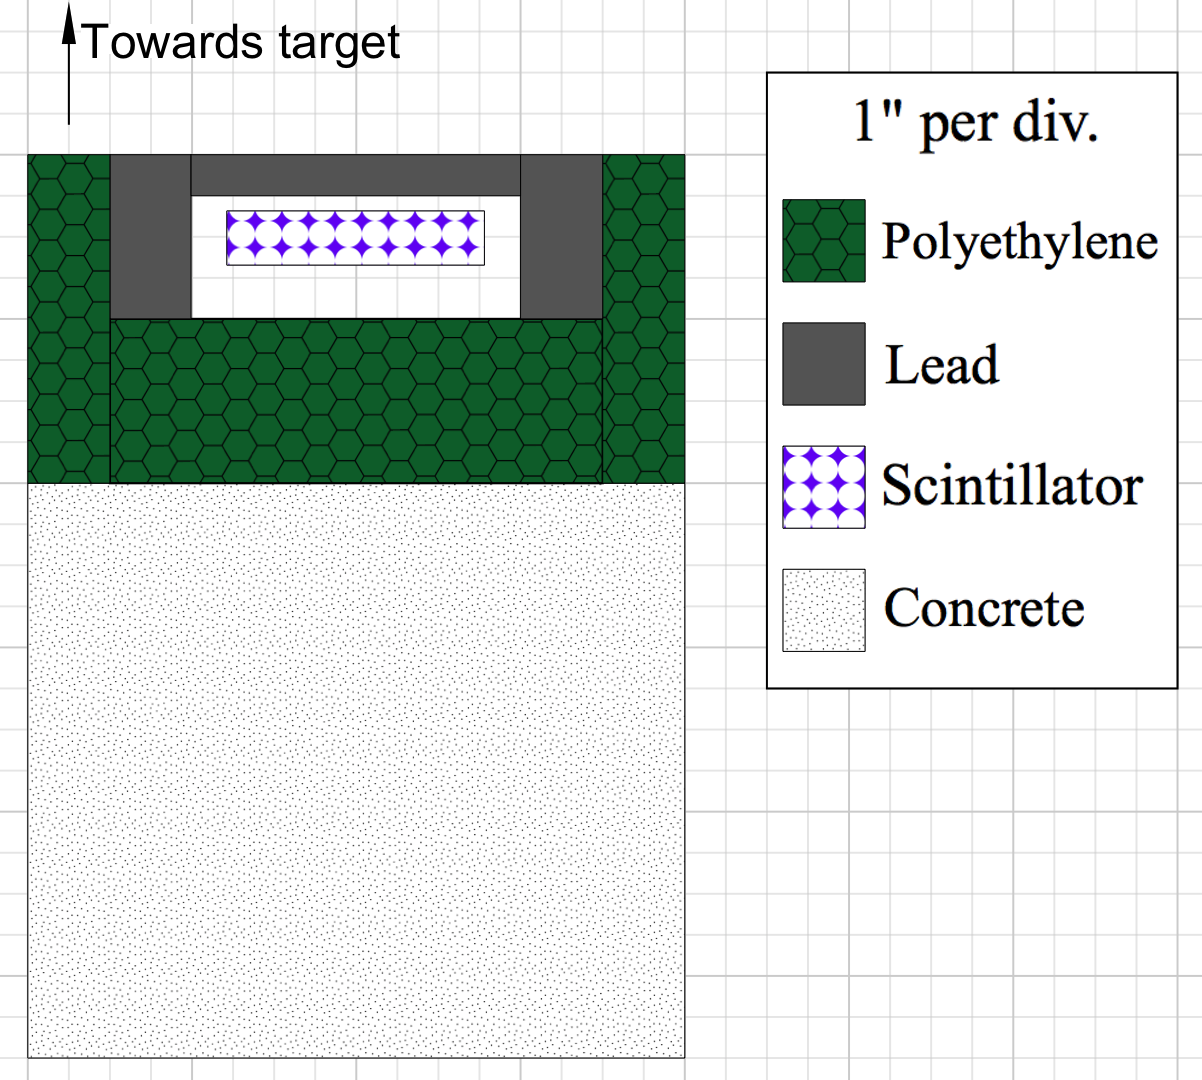
\includegraphics[width = 0.65\textwidth]{Content/Methods/DetShielding.png}
    \caption{Detector shielding was designed to reduce the detection of photons, room return, and detector cross-talk.}
    \label{fig:shielding}
\end{figure}

\subsection{Bremsstrahlung Photon Beam}
\label{beam}
In order to ensure that all correlated neutrons produced are due to fission, the bremsstrahlung end-point was set to 10.5~MeV, safely below the ($\gamma, 2n$) threshold of 11.28~MeV for $^{238}$U.
Al was chosen for a bremsstrahlung radiator because it has a neutron knockout threshold above the energy of the electron beam, which ensured that the radiator would not be a source of fast neutrons with the potential to interfere with the experiment.
Downstream from the bremsstrahlung radiator is a sweeping magnet that removes charged particles from the photon beam.
Next, the beam traveled through a series of polyethylene and lead collimators on its way into the experimental cell in which the target was located (see Fig.~\ref{fig:Facility}).
Figure~\ref{fig:BremDist} shows the energy distribution of photons that reach the target according to an MCNP simulation that included the production and collimation of the bremsstrahlung photon beam.

The electron beam pulse width was set to 3~ns with a repetition rate of 240~Hz and a 1.1~A peak current.
The 3~ns pulse width was small compared to the median neutron ToF of 80~ns, and thus made a small contribution to the uncertainty in the neutron energy determination.

\begin{figure}[h]
\centering
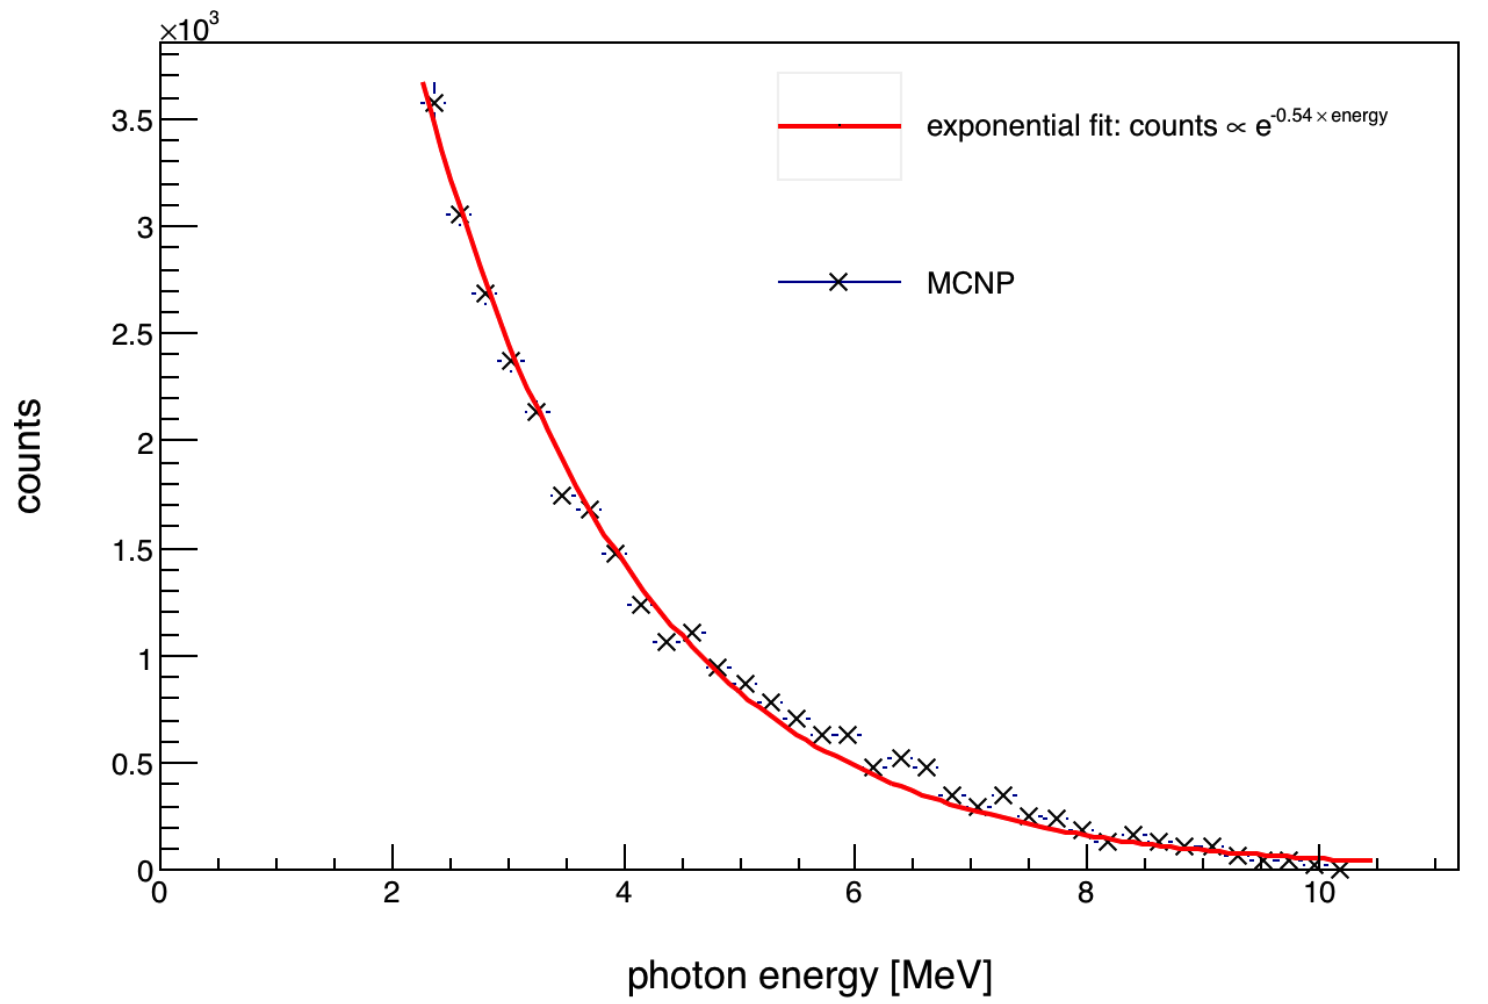
\includegraphics[width=0.7\textwidth]{Content/Methods/MCNPBremDistribution.png}
\caption{MCNP simulation of the energy distribution of photons that are incident on the fission target.}
\label{fig:BremDist}
\end{figure}

\subsection{DU Target}
\label{subsection:targets}
\begin{figure}[]
\centering
    \subfloat[]{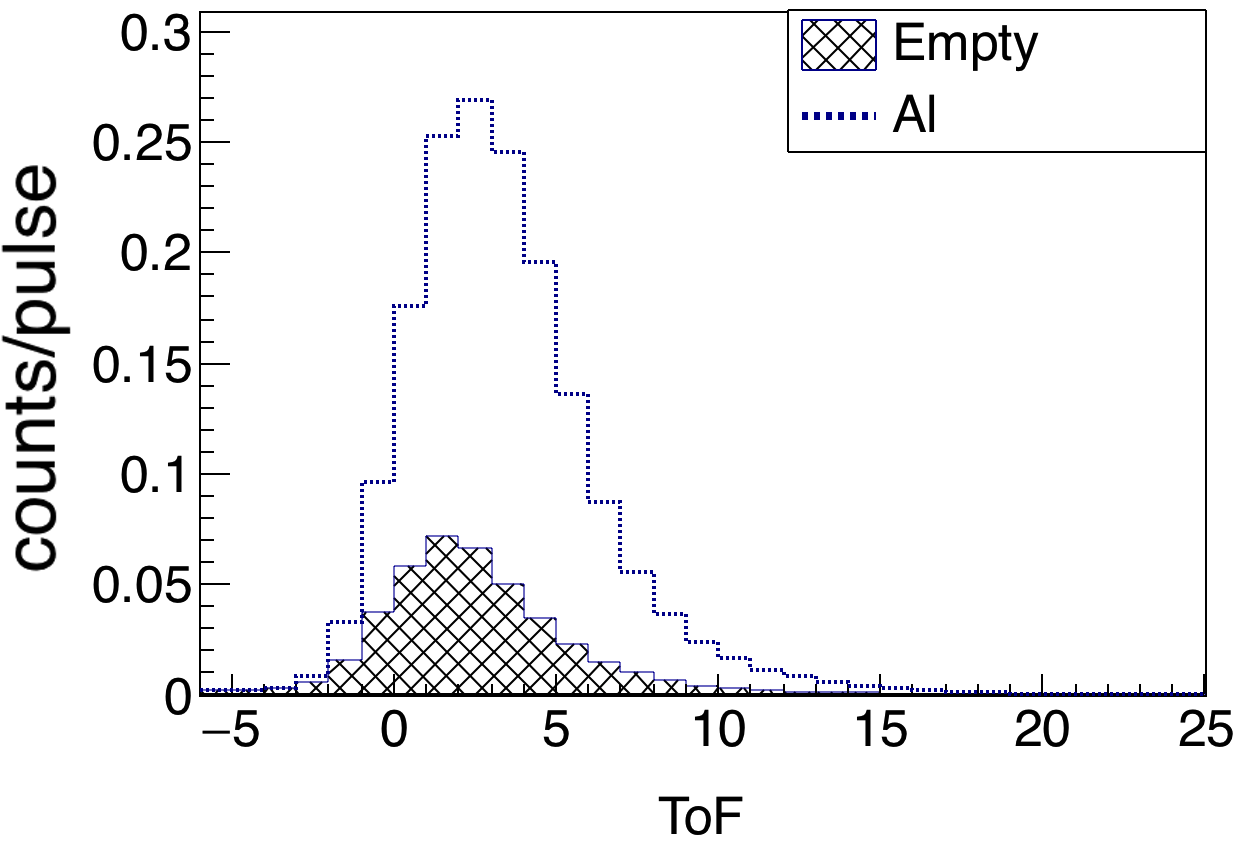
\includegraphics[width=0.5\textwidth]{Content/Methods/MTvsAl.png}}
    \subfloat[]{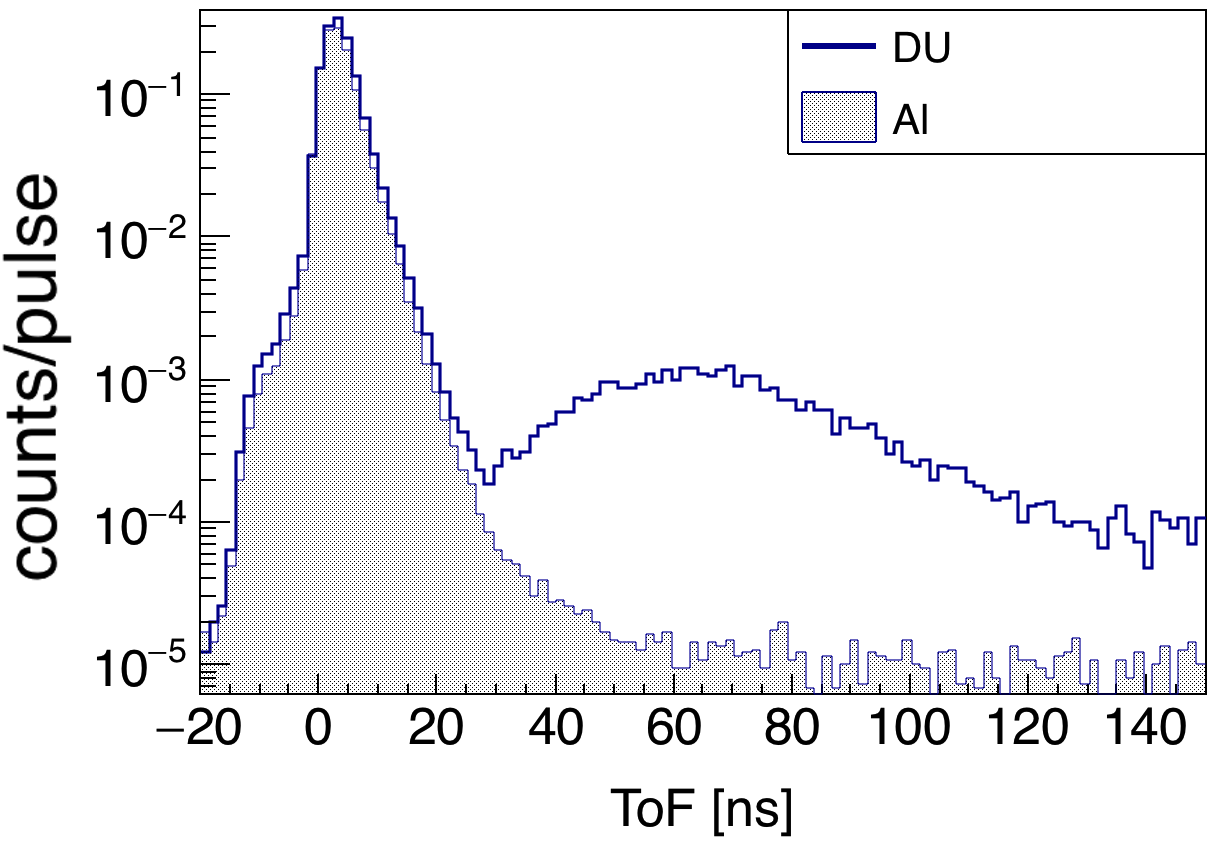
\includegraphics[width=0.5\textwidth]{Content/Methods/DUvsAl.png}}
    \caption{(a) Comparison between the ToF spectrum of a non-neutron producing target made from Al, to the ToF spectrum produced when no target is used.
    The large increase in events around 4~ns is due to photons that scatter from the Al target.
    When no target is in place, sources of the peak include the collimator leading into the experimental cell and the beam dump.
    The photon peak seen here is used to find the timing offsets that make it so $t=0$ corresponds to the moment of fission.
    (b) Comparison between the Al and DU targets show a pronounced increase in events between 35 and 130~ns due to the introduction of neutrons.}
    \label{fig:ToF}
\end{figure}
A depleted uranium (DU) target in the shape of a thin strip with dimensions of 4$\times$2$\times$0.05 $\text{cm}^3$ was used as the primary target.
U-238 received the majority of allotted beam time because it is an even-even nucleus, and as a consequence, the fission fragments are emitted with a high degree of anisotropy~\cite{1977FragAss}.

Any target comprised of heavy nuclei has a significant potential to scatter fission neutrons before they exit the target, which is a cause for concern, because neutrons that scatter from heavy nuclei are likely to be deflected at large angles, facilitating the measurement of $\theta_{nn}$'s unconnected to the underlying fission kinematics.
The rate of $\theta_{nn}$'s perturbed by neutron scattering within the $^{238}$U target was estimated by an MCNP simulation to be 6\%.
Moreover, it is more likely that neutrons emitted along the wide, 2~cm, axis of the $^{238}$U target undergo a scattering event than neurons emitted along the thinest, 0.05~cm, axis.
As a result, detectors located collinear to the widest axis of the target would see relatively fewer neutrons due to increased scattering along this axis. 
This bias is removed by slowly rotating the target about the vertical axis during data acquisition.
Because the subject of this measurement is fundamentally a statistical process, useful interpretations of the data are average rates taken over many events.
Thus, by rotating the target, cylindrical symmetry is preserved in the average to produce a result much the same to that if a cylindrical target were used.
See section~\ref{subsection:Elastic_scattering} for details about all issues regarding neutron scattering with the fission target.  

\subsection{Electronics}
A data acquisition system based on NIM/VME standard was used.
A schematic of the data acquisition logic is shown in Figure~\ref{fig:WiringDiagram}.
The PMTs are supplied negative voltages ranging from 1300 to 1500 V by a LeCroy 1458 high voltage mainframe.
Analog signals from the PMTs were fed into a leading edge discriminator (CAEN Mod. N841) with input thresholds ranging from 30 mV to 50 mV.
The threshold and supply voltages were determined on a case by case basis for each detector so as to minimize noise, while also matching the efficiencies of all the detectors as closely as possible.
Logic signals from the discriminator were converted to ECL logic and fed into a CAEN model V1290A TDC.
The timing of signals from the PMTs were always measured relative to a signal from the accelerator provided at the beginning of each pulse.
Even though a multi-hit TDC was being used, only the first signal from any given PMT is used each pulse due to concerns over dead-time within the electronics and signal reflections within the cables.
On the software side, the CODA~\cite{CODA} software package developed by Jefferson Laboratory was used to read out the data from the TDC and digitally store it for analysis.

\begin{figure}[h]
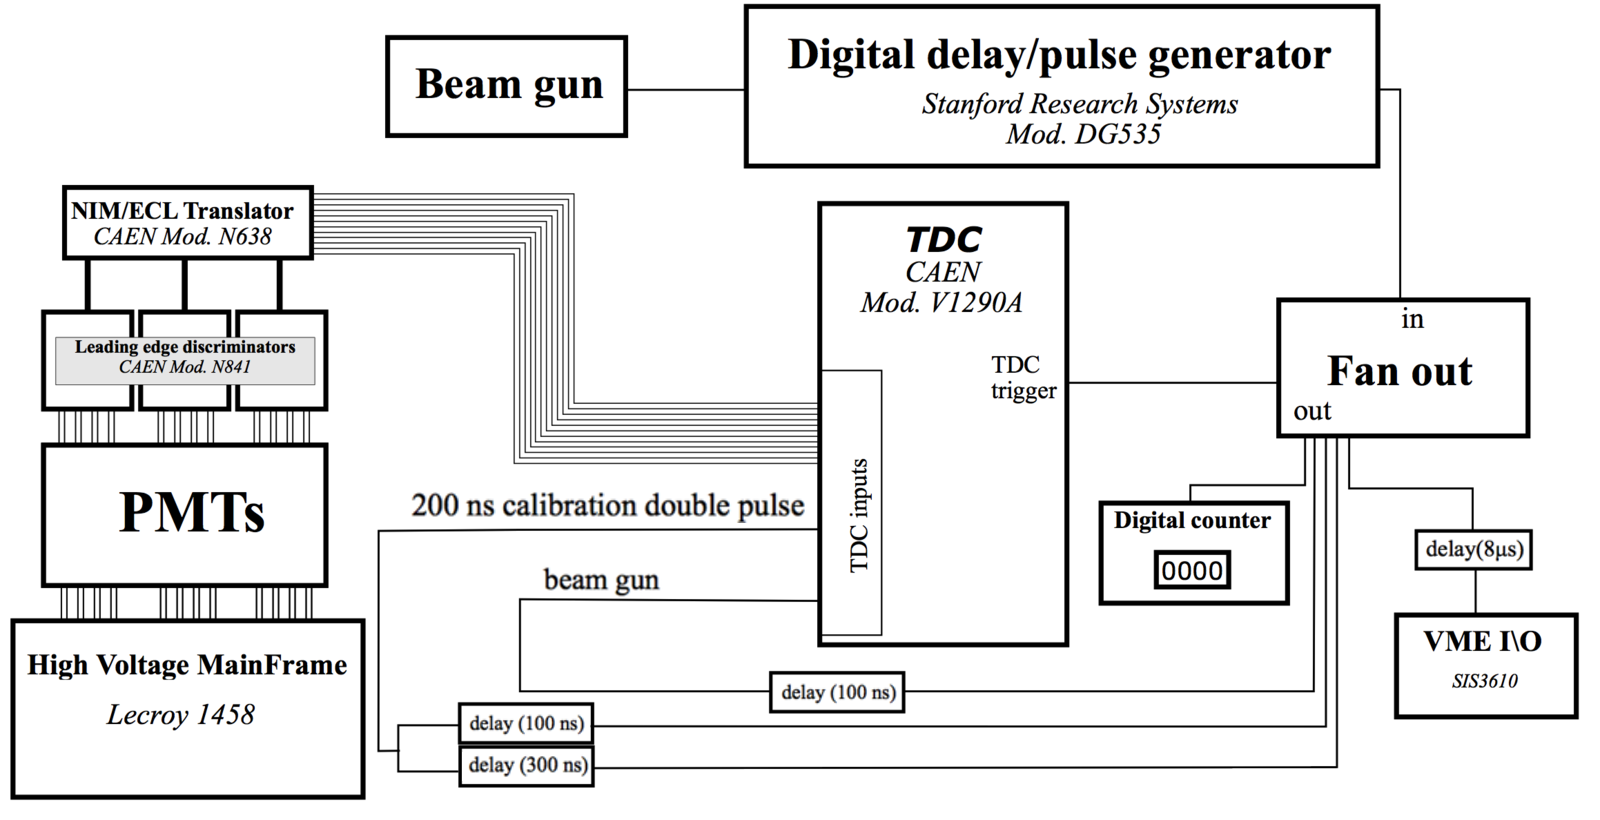
\includegraphics[width=0.9\textwidth]{Content/Methods/WiringDiagram.png}
\caption{Wiring diagram of the electronics setup. }
\label{fig:WiringDiagram}
\end{figure}
